\documentclass[border=4pt]{standalone}
% Shared style for every diagram. Colour-blind-safe palette (Okabe-Ito).
\usepackage[T1]{fontenc}
\usepackage{helvet}
\renewcommand{\familydefault}{\sfdefault}
\usepackage{tikz}
\usetikzlibrary{arrows.meta,positioning,fit,backgrounds,calc,shapes.geometric,decorations.pathreplacing}
\definecolor{cblue}{HTML}{0072B2}
\definecolor{corange}{HTML}{E69F00}
\definecolor{cgreen}{HTML}{009E73}
\definecolor{cred}{HTML}{D55E00}
\definecolor{cpurple}{HTML}{CC79A7}
\definecolor{cgrey}{HTML}{6B7280}
\definecolor{csky}{HTML}{56B4E9}
\tikzset{
  >={Stealth[length=2.2mm]},
  box/.style={draw, rounded corners=3pt, align=center, minimum height=11mm, minimum width=22mm, font=\small, line width=0.7pt},
  real/.style={box, draw=cblue, fill=cblue!8},
  sim/.style={box, draw=corange, fill=corange!12},
  future/.style={box, draw=cgrey, dashed, fill=white},
  flow/.style={->, line width=0.8pt, draw=black!75},
  dflow/.style={->, line width=0.8pt, dashed, draw=cgrey},
  lbl/.style={font=\scriptsize, text=black!70},
  group/.style={draw=black!25, rounded corners=6pt, inner sep=6pt},
}

\begin{document}
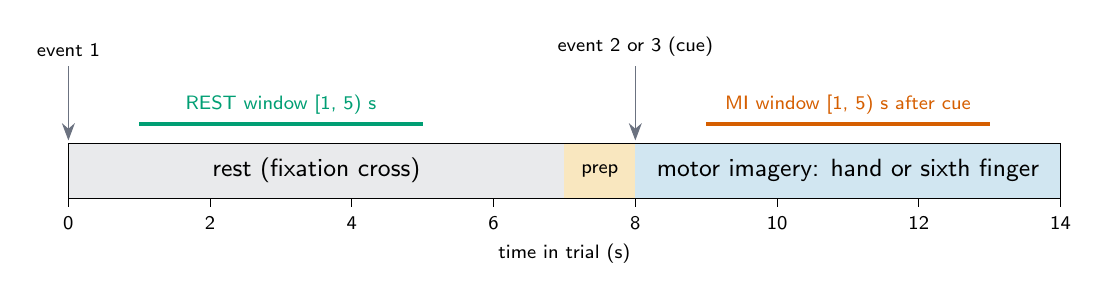
\begin{tikzpicture}[x=9mm, y=7mm]
  \fill[cgrey!15] (0,0) rectangle (7,1);   \node[font=\small] at (3.5,0.5) {rest (fixation cross)};
  \fill[corange!25] (7,0) rectangle (8,1); \node[font=\scriptsize] at (7.5,0.5) {prep};
  \fill[cblue!18] (8,0) rectangle (14,1);  \node[font=\small] at (11,0.5) {motor imagery: hand or sixth finger};
  \draw (0,0) rectangle (14,1);
  \foreach \t in {0,2,...,14} { \draw (\t,0) -- (\t,-0.15) node[below, font=\scriptsize] {\t}; }
  \node[font=\scriptsize] at (7,-1.0) {time in trial (s)};
  \draw[very thick, cgreen] (1,1.35) -- (5,1.35);
  \node[font=\scriptsize, text=cgreen, above] at (3,1.35) {REST window [1, 5) s};
  \draw[very thick, cred] (9,1.35) -- (13,1.35);
  \node[font=\scriptsize, text=cred, above] at (11,1.35) {MI window [1, 5) s after cue};
  \draw[->, cgrey] (0,2.4) node[above, font=\scriptsize, text=black] {event 1} -- (0,1.05);
  \draw[->, cgrey] (8,2.4) node[above, font=\scriptsize, text=black] {event 2 or 3 (cue)} -- (8,1.05);
\end{tikzpicture}
\end{document}
